\section{Karazhan}

\subsubsection{About the zone}

Karazhan\footnote{The design for this is from World of Warcraft, the contents are, however, very different.} is a large castle in the Pluvian Forest. It is home to yaga. The castle is huge and contains many rooms. There is a great deal of information, treasures, spell scrolls and more that the players can find in here. There are also puzzle rooms, trap rooms and normal rooms.

\begin{center}
	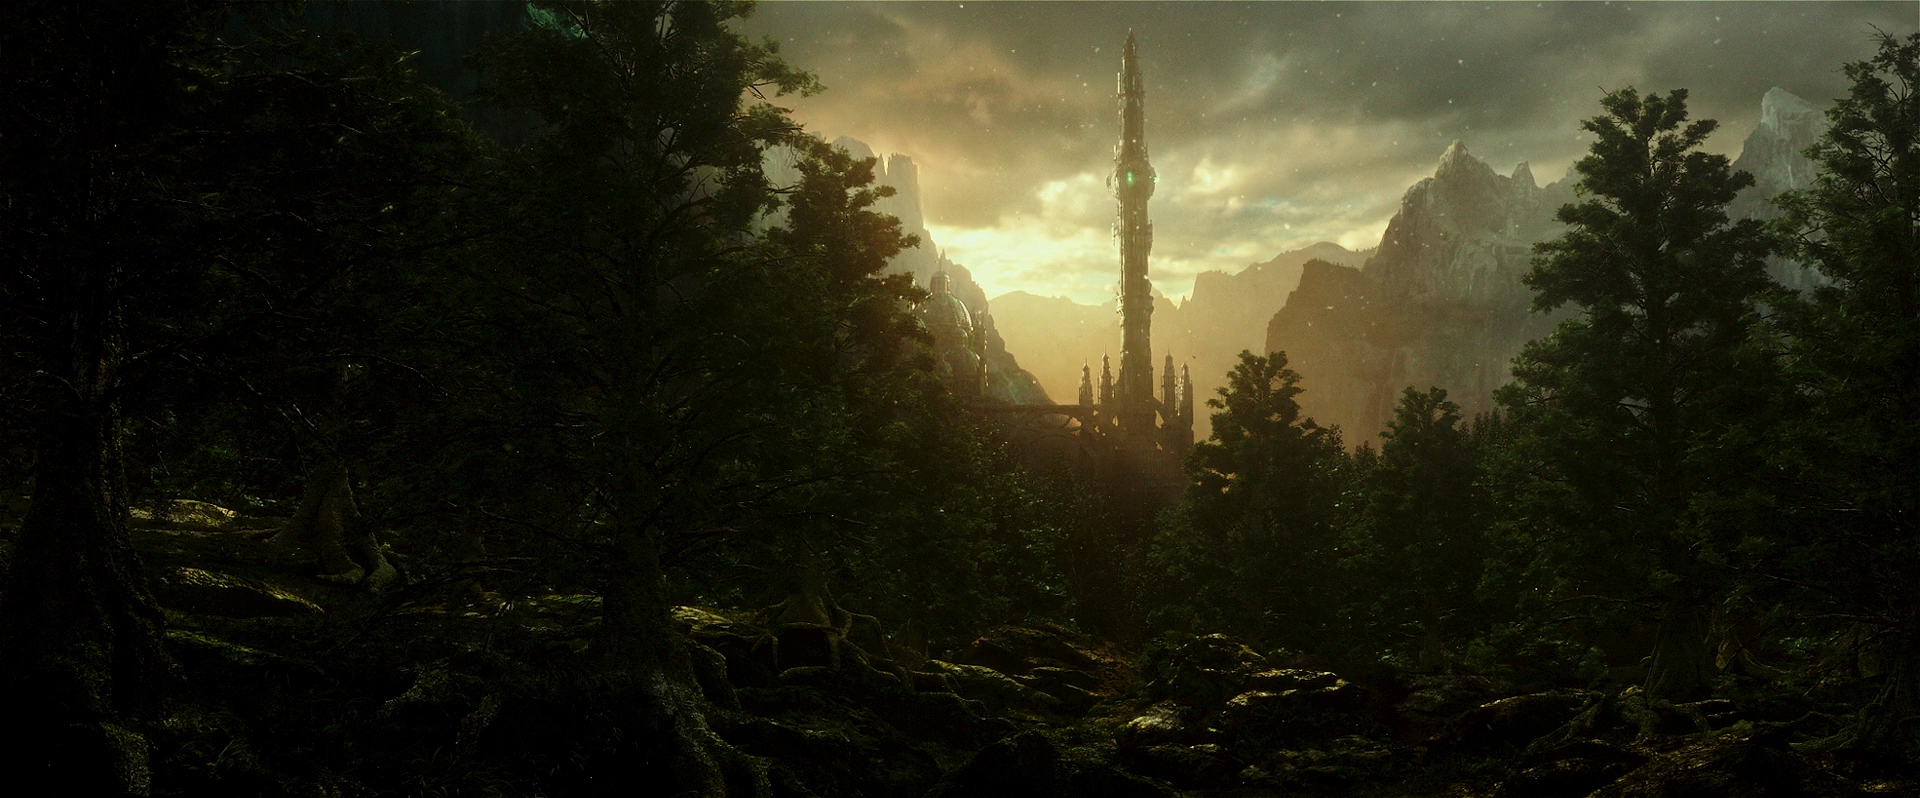
\includegraphics[width=0.99\textwidth]{img/Karazhan/9bI9O27.jpg}
\end{center}

\begin{center}
	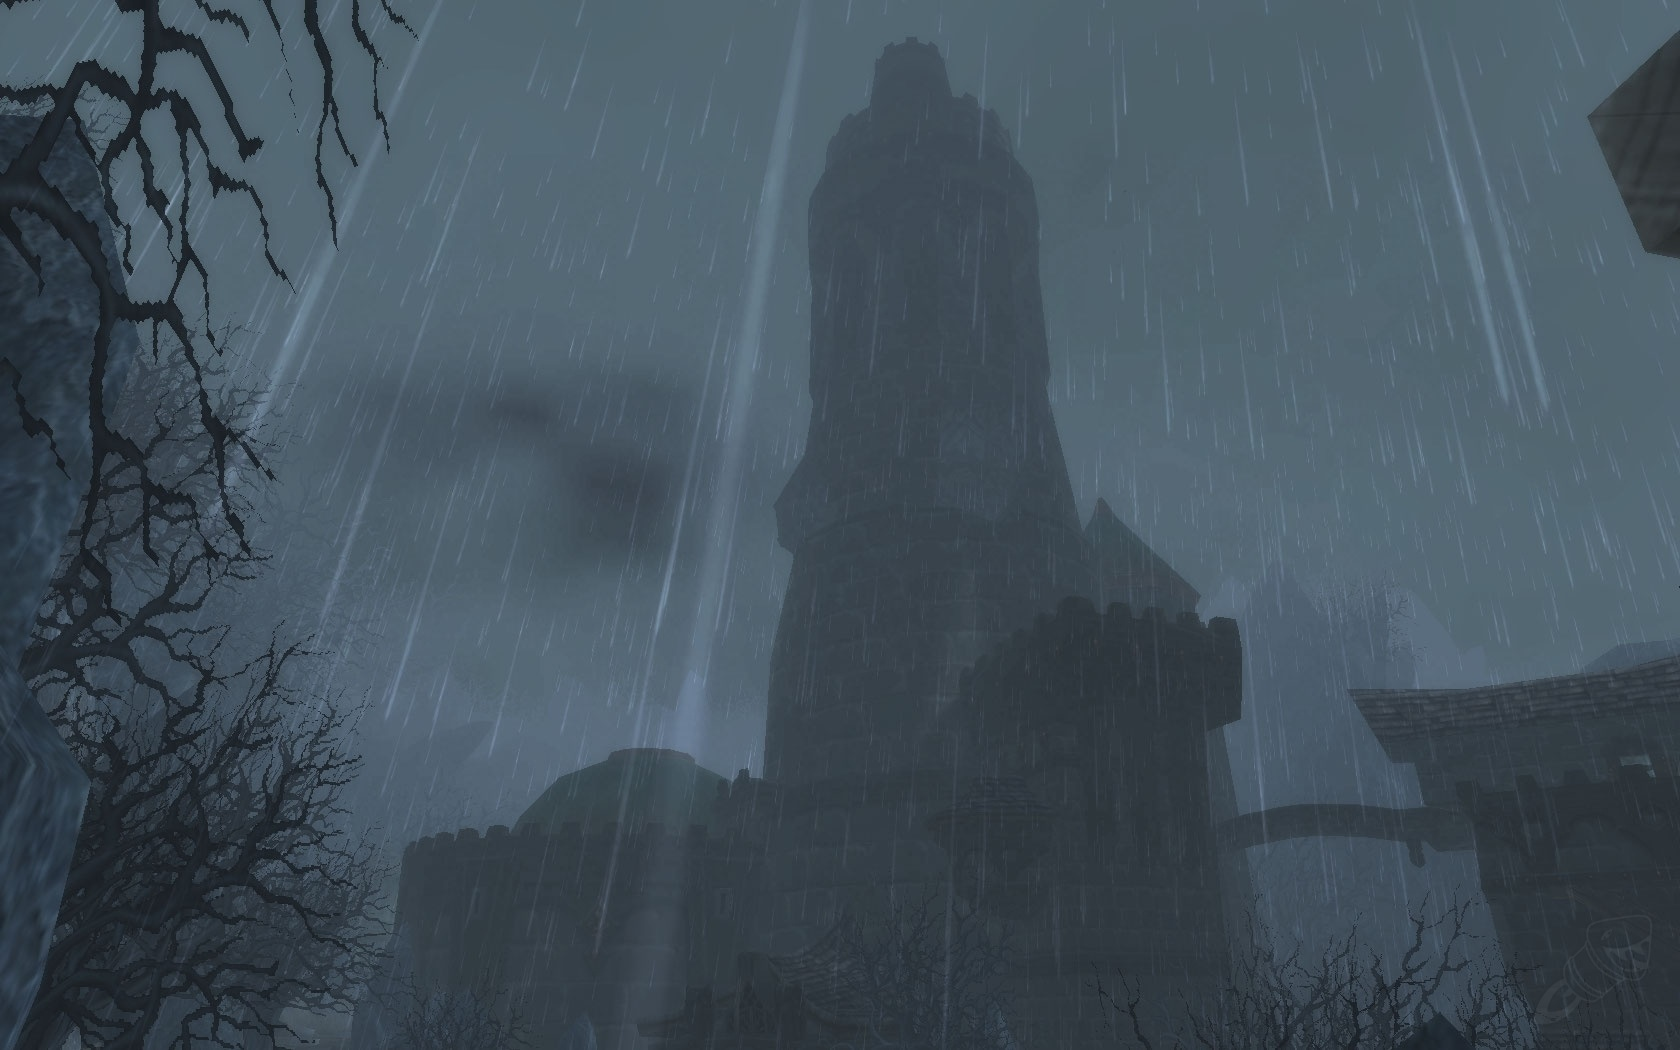
\includegraphics[width=0.41\textwidth]{img/Karazhan/175259-karazhan.jpg} 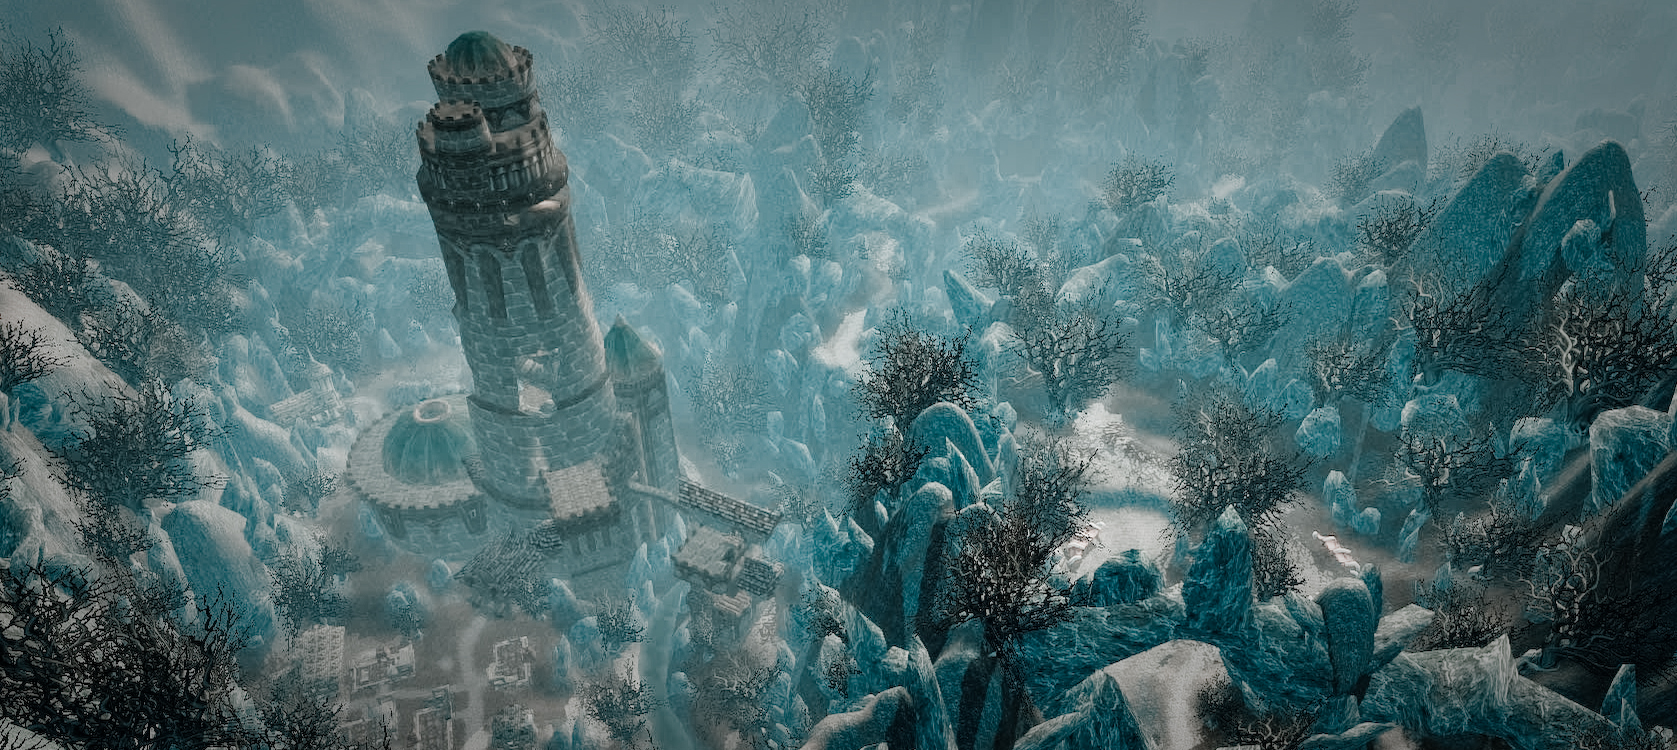
\includegraphics[width=0.57\textwidth]{img/Karazhan/karazhan.jpg}
\end{center}

Throughout the area, there is a faint music that plays which is louder towards the opera hall. The music is from a ghost that is playing an organ. The ghost will make no notice of the party but will continue to play the organ continually. He cannot interact with the party physically, but only the organ itself.

\subsubsection{Entrance and Livery Stables}

There are two entrances to karazhan. The main entrance is an open gate with a large wooden door at the front steps of the castle. The secondary entrance is across a large bridge up on the secondary tower next to the main castle structure. The players can enter from either place. 

Upon entering the front main door, the party sees a large room that breaks off into three directions. To the right they see a large staircase and to the left a large doorway leading into what appears as a stabling area (the Livery Stables) for horses. Right next to where they are to the right they also see what leads off into what could be catacombs but is actually the servants quarters. The Livery Stables contain the remains of dead horse corpses but also contain horse ghosts that roam the area. They are connected to the kitchen area and food storage areas.

\begin{center}
	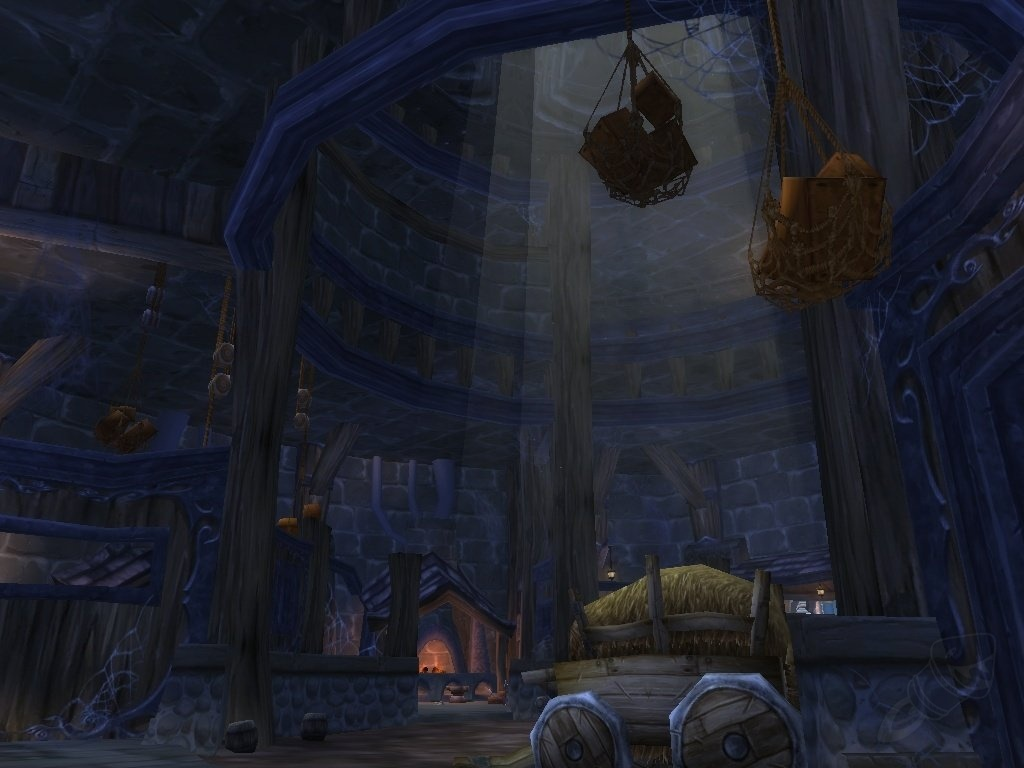
\includegraphics[width=0.37\textwidth]{img/Karazhan/21972-karazhan-the-livery-stables-this-is-where-you-fight-attumen-the-huntsman.jpg} 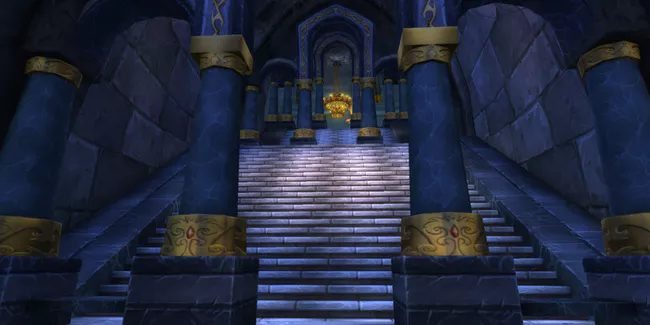
\includegraphics[width=0.56\textwidth]{img/Karazhan/karazhansteps.jpg}
	
	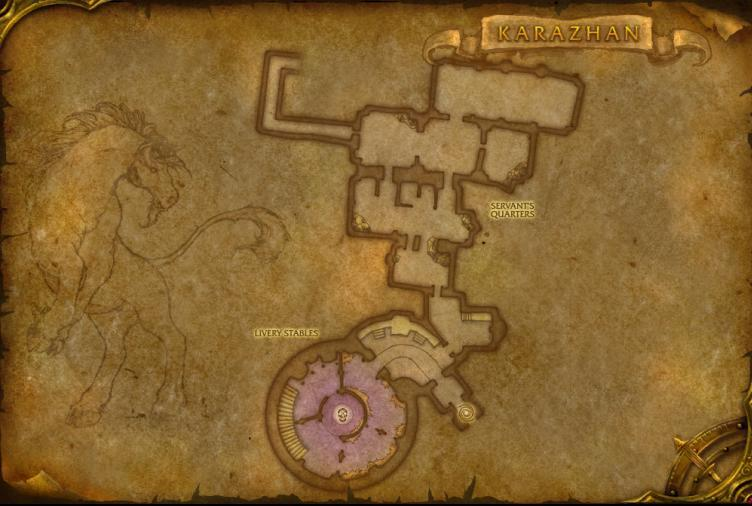
\includegraphics[width=0.46\textwidth]{img/Karazhan/cropped-3457-1.jpg} 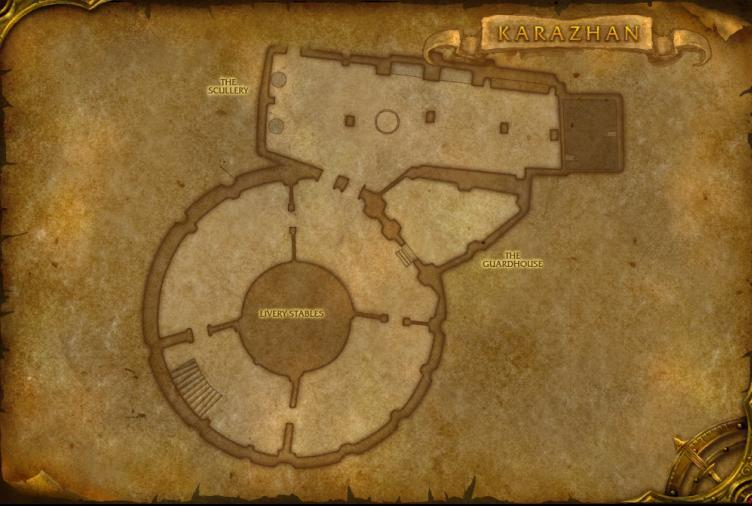
\includegraphics[width=0.46\textwidth]{img/Karazhan/cropped-3457-2.jpg}
\end{center}

The back door, the one on across the bridge, opens up to a different broken down region much higher up in the tower.

\begin{center}
	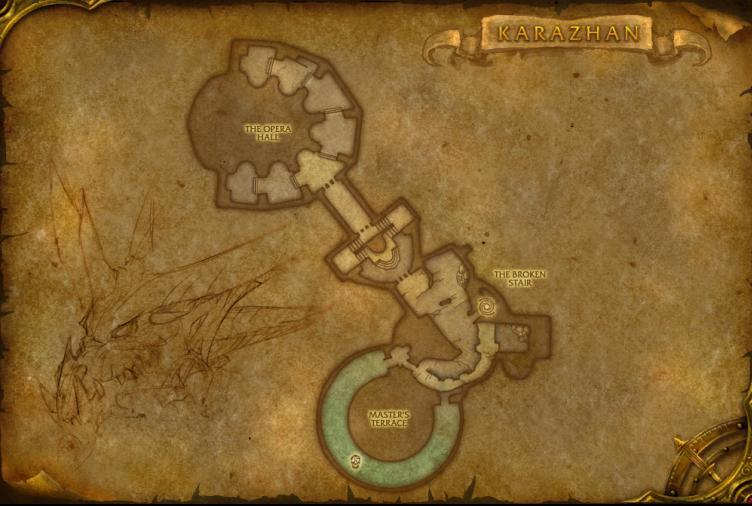
\includegraphics[width=0.48\textwidth]{img/Karazhan/cropped-3457-6.jpg}
	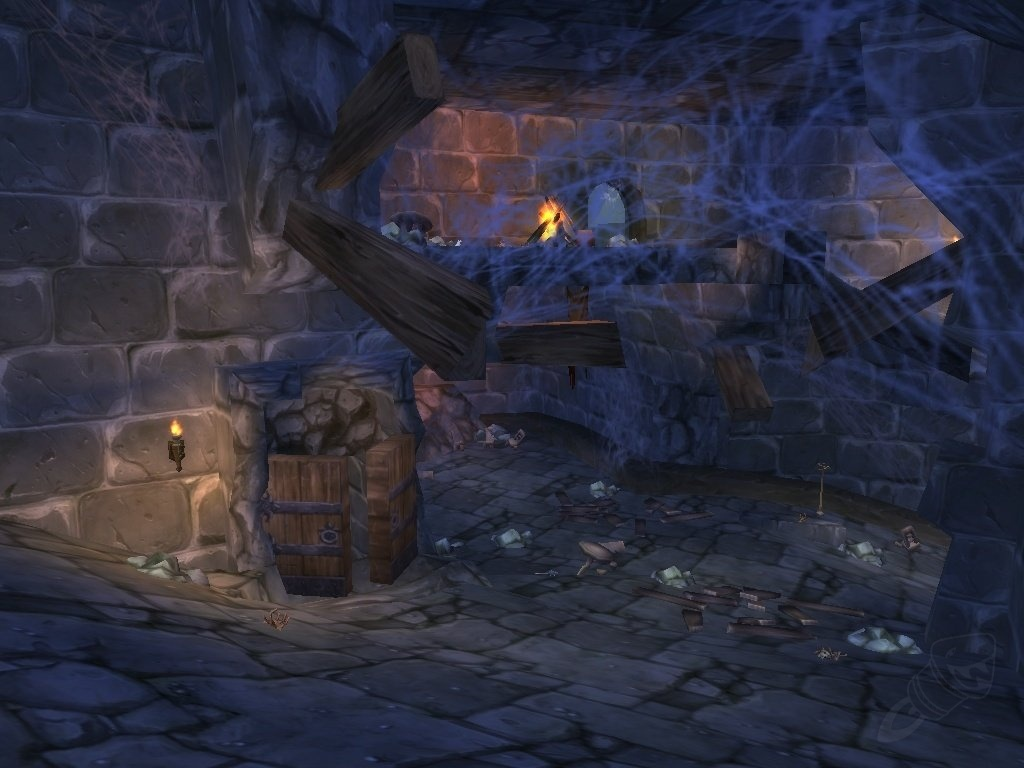
\includegraphics[width=0.43\textwidth]{img/Karazhan/21983-karazhan-the-back-entrance-if-youve-cleared-the-opera-you-can-enter-the-instance.jpg}
\end{center}

\subsubsection{The Royal Ballroom and Opera Hall}

If the players leave the entrance by way of stairway, they will enter the royal ballroom. This ballroom is a large area with many non-hostile ghosts dancing as if stuck this way. The ballroom has a staircase leading to a higher level connected to the ballroom and also has a stairway leading into a dining area. 

\begin{center}
	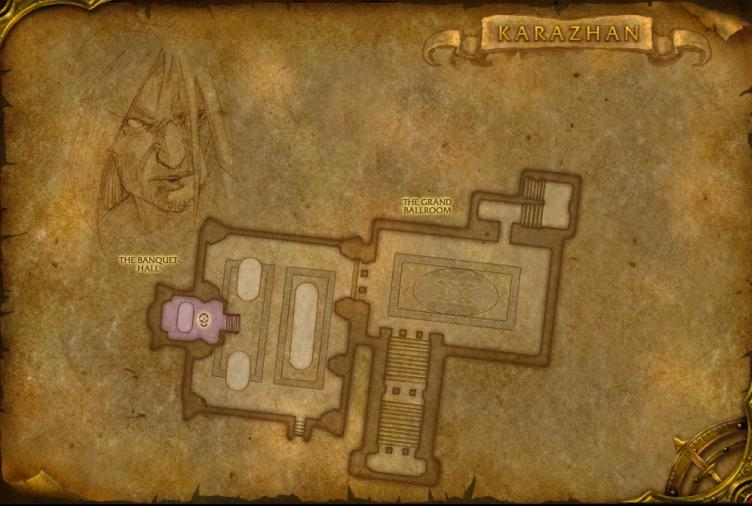
\includegraphics[width=0.45\textwidth]{img/Karazhan/cropped-3457-3.jpg} 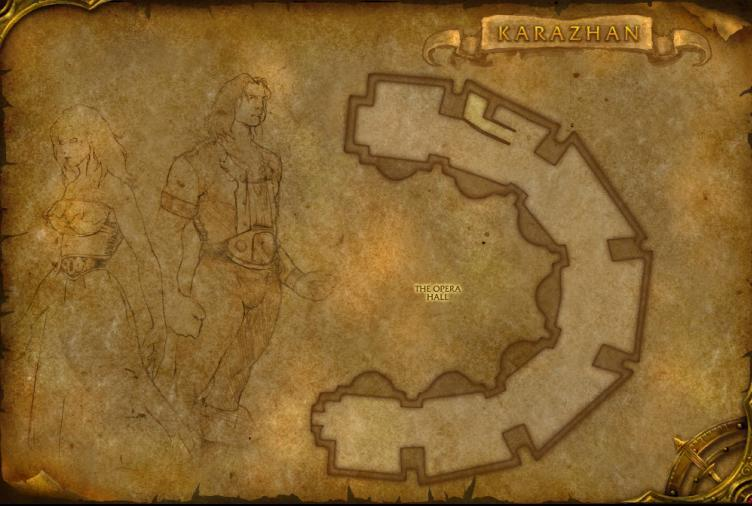
\includegraphics[width=0.45\textwidth]{img/Karazhan/cropped-3457-5.jpg}
	
	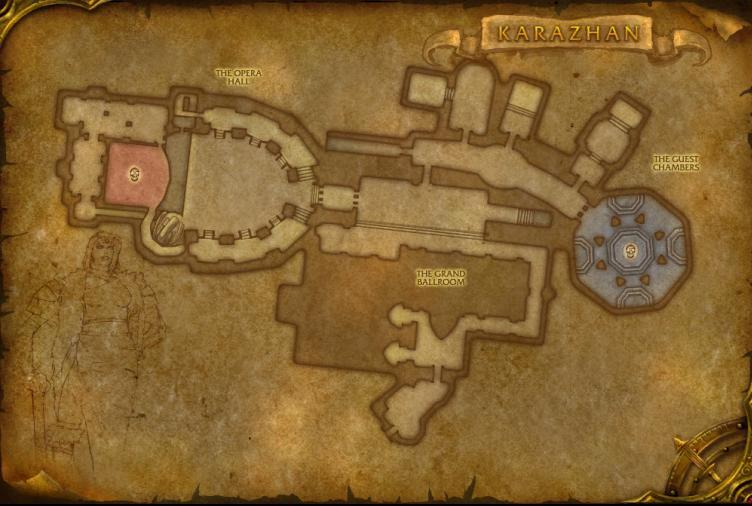
\includegraphics[width=0.90\textwidth]{img/Karazhan/cropped-3457-4.jpg}
\end{center}

\subsubsection{The Broken Stairs}

This is a region that is between the Master's Terrace and The Menagerie. Is is a broken area with stairs leading to an upper level.

\begin{center}
	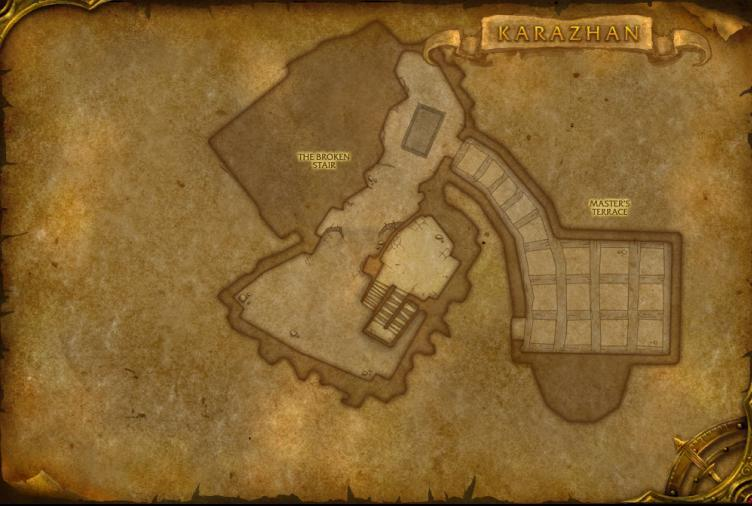
\includegraphics[width=0.45\textwidth]{img/Karazhan/cropped-3457-7.jpg} 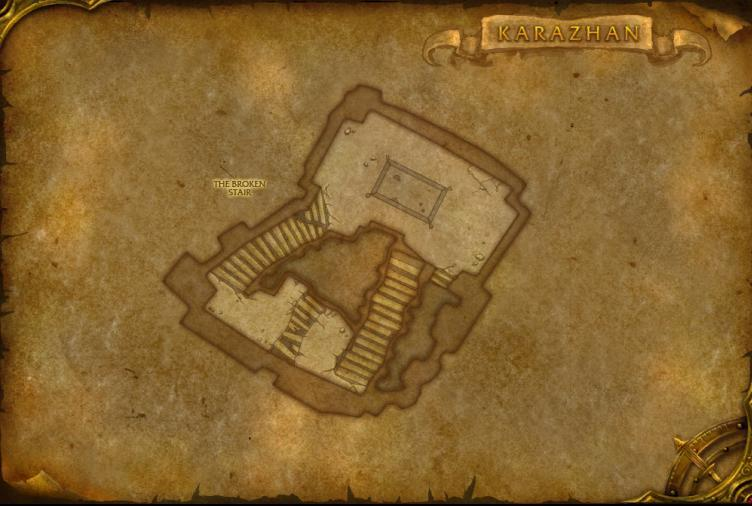
\includegraphics[width=0.45\textwidth]{img/Karazhan/cropped-3457-8.jpg}
\end{center}

\subsubsection{The Menagerie and The Guardians Library}

The Menagerie is a magical at the entrance of the guardians library. The Menagerie is home to the Curator which is a magically advanced being that can assist the players through the guardians library. The curator is extremely powerful but is non-hostile unless it is attacked or it has to protect Karazhan and the contents of the library.

\begin{commentbox}{The Curator}
	The curator will come alive when the party enters The Menagerie. He is sleeping at first, but will activate and become fully alive. He is very knowledgeable and knows all of the material in the library surrounding them. 
	
	\begin{center}
		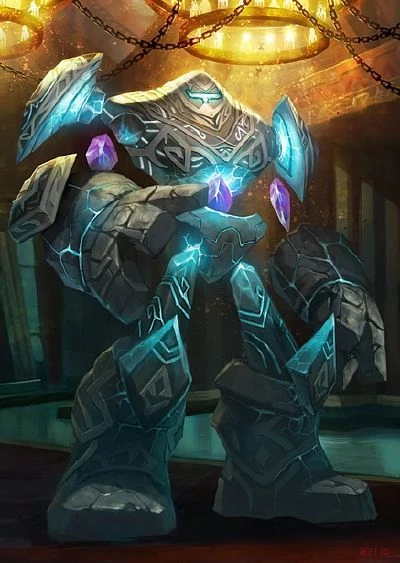
\includegraphics[width=0.17\textwidth]{img/Karazhan/400px-The_Curator_full.jpg} 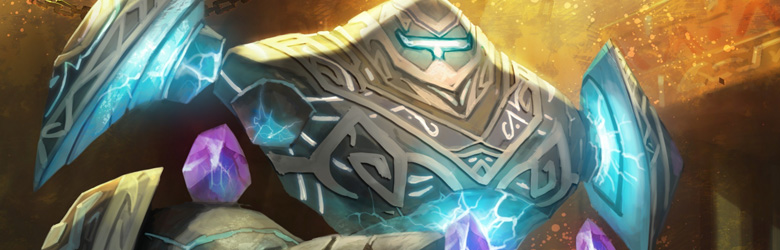
\includegraphics[width=0.74\textwidth]{img/Karazhan/featured-thecurator.jpg}
	\end{center}
\end{commentbox}

\begin{monsterbox}{The Curator}
	\begin{hangingpar}
		\textit{Large Construct, Neutral Good}
	\end{hangingpar}
	\dndline%
	\basics[%
	armorclass = 20,
	hitpoints  = 234,
	speed      = 30 ft
	]
	\dndline%
	\stats[
	STR = \stat{24}, % This stat command will autocomplete the modifier for you
	DEX = \stat{18},
	CON = \stat{21},
	INT = \stat{30},
	WIS = \stat{16},
	CHA = \stat{20}
	]
	\dndline%
	\details[%
	% If you want to use commas in these sections, enclose the
	% description in braces.
	% I'm so sorry.
	languages = {All},
	challenge = 10
	]
	\dndline%
	\begin{monsteraction}[Telekinesis]
		The ability to move objects with your mind. There is no limitation to how the objects can be moved if the objects belong to you.
	\end{monsteraction}	
	\begin{monsteraction}[Magical Resistance]
		You are resistance to all magic.
	\end{monsteraction}	
	\begin{monsteraction}[Static Charged Elements]
		Your body contains surging electrical flow. When you are struck by a melee attack the attacker takes 1d4 damage.
	\end{monsteraction}
	\monstersection{Actions}
	\begin{monsteraction}[melee attack]
		melee attack: +6 to hit. 2d10+3 bludgeoning damage. 
	\end{monsteraction}
	\begin{monsteraction}[Menagerie Void Creatures]
		You can create any number of menagerie void creatures to send after your opponents.
	\end{monsteraction}
\end{monsterbox}

\begin{commentbox}{Menagerie Void Forms}
	 The Menagerie void forms are humanoid like beings surrounded in cerebral void energy. These creatures have very limited interaction capabilities from the immediate dimension. These creatures can charge a creature and push it's spirit temporarily out of it's body. When done, the creature can enter an illusion that it must escape from before being able to return to its body. One such illusion is that the player must fight a skeletal mimic of themselves (mimicking all their abilities) and win.
	
	\begin{center}
		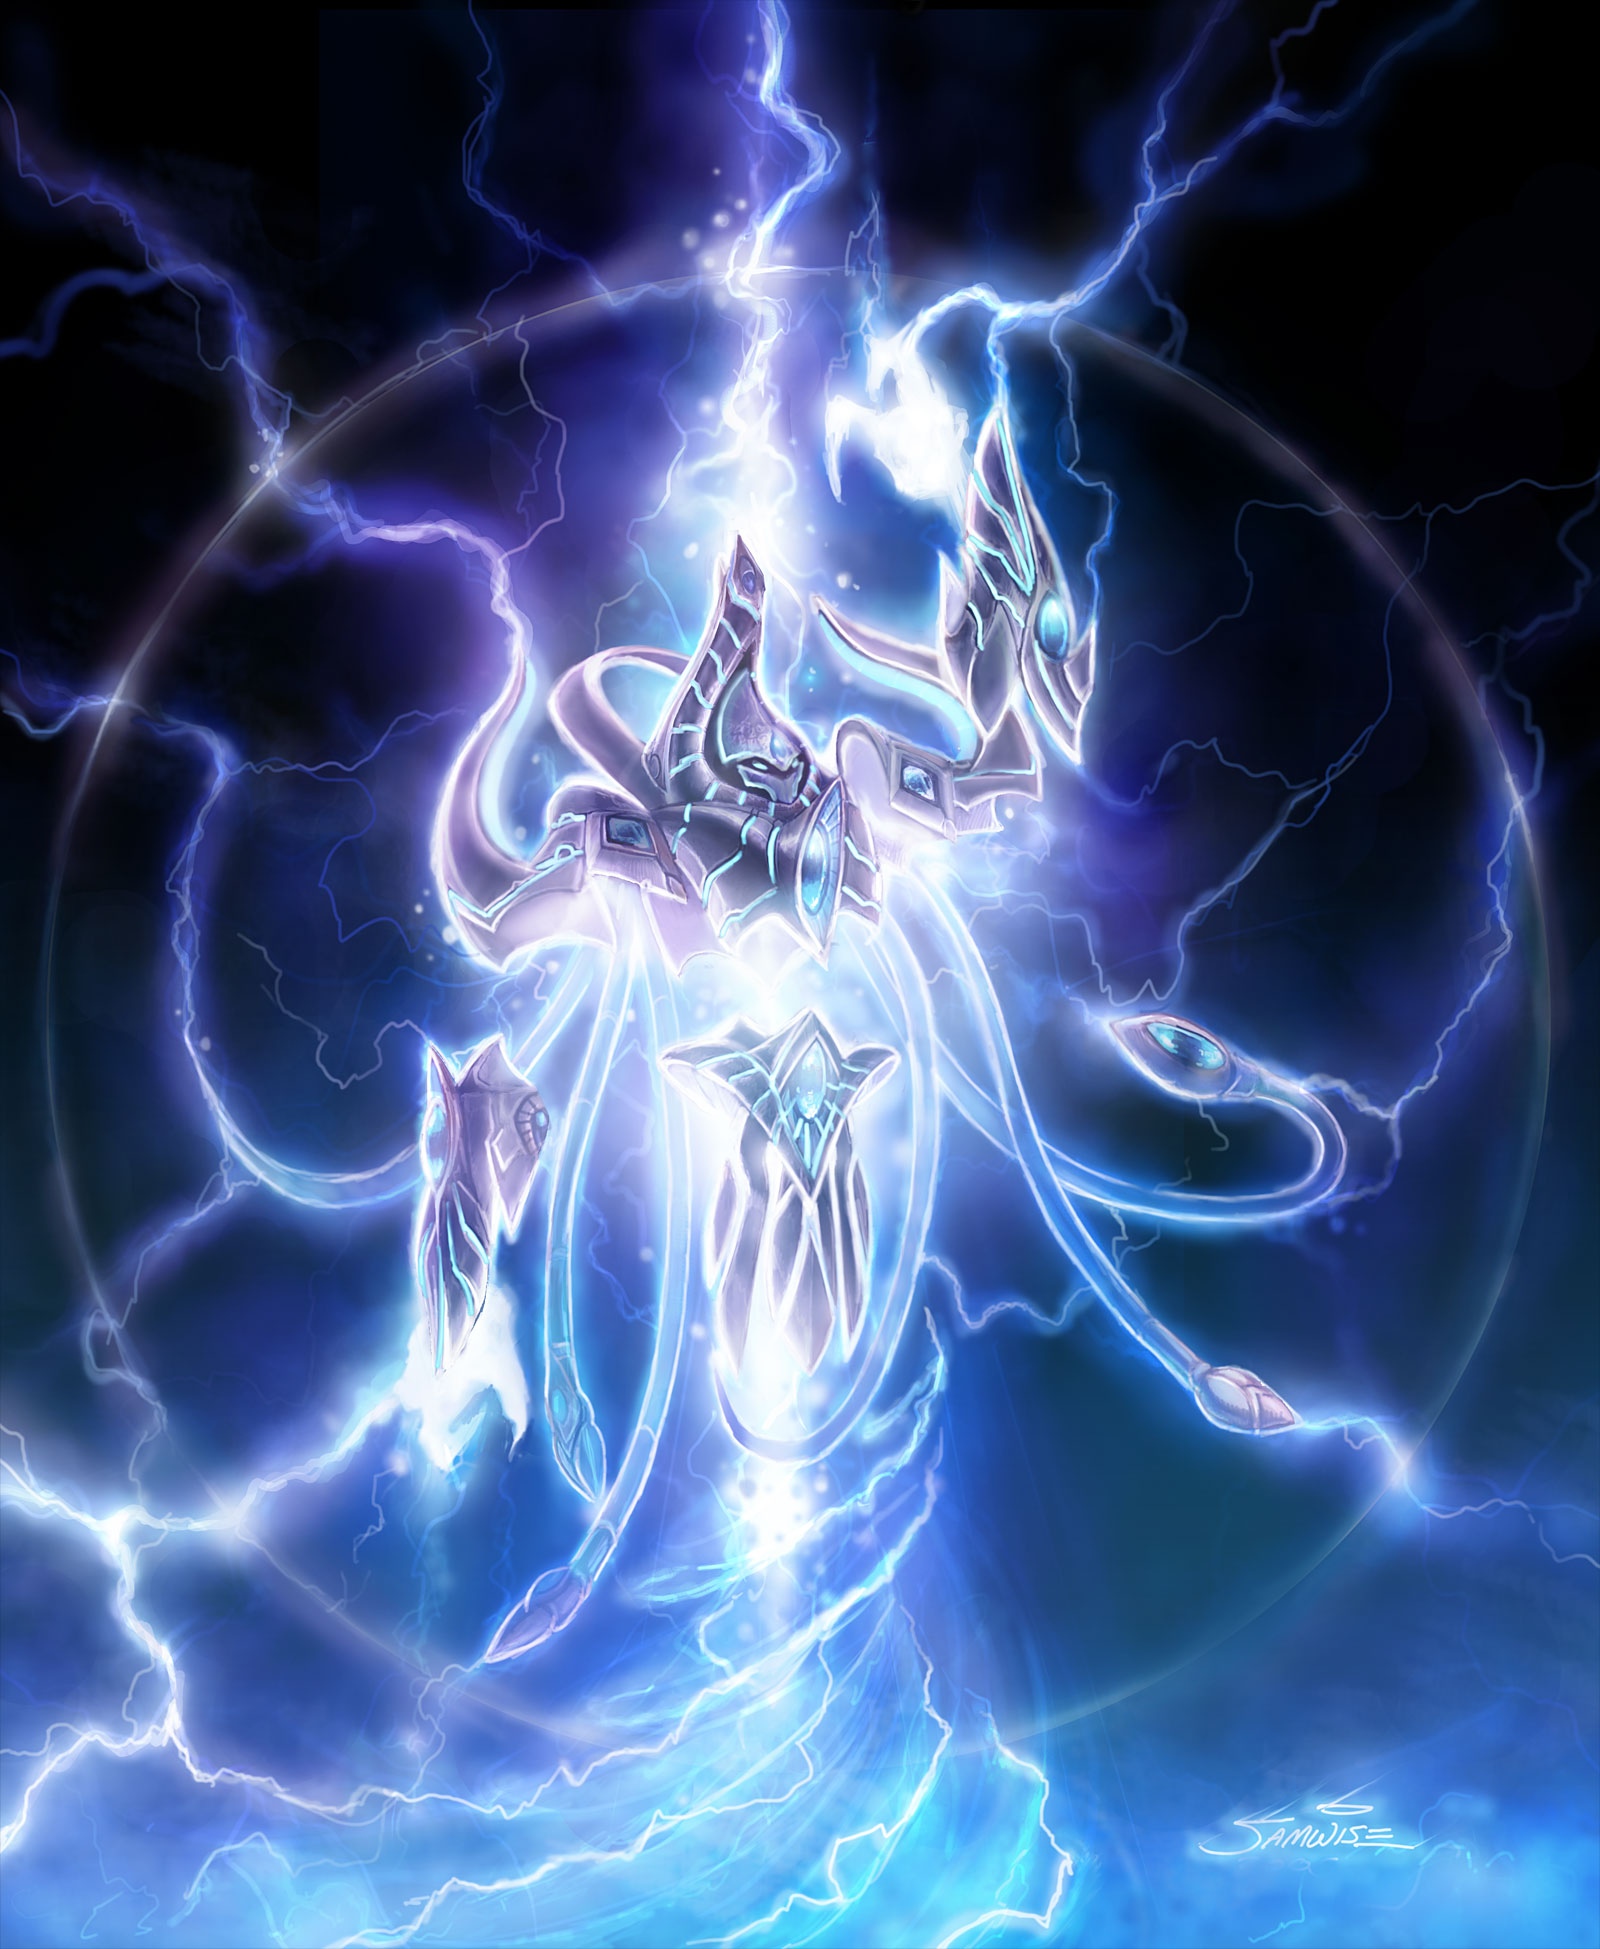
\includegraphics[width=0.38\textwidth]{img/Karazhan/ss26-hires.jpg} 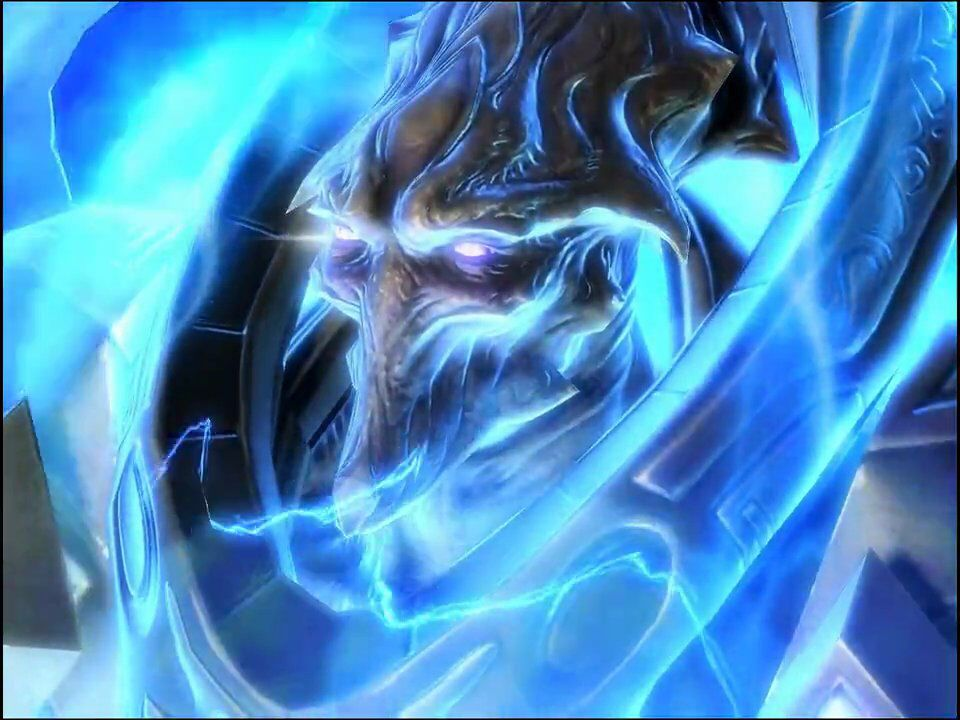
\includegraphics[width=0.61\textwidth]{img/Karazhan/9640b2f687a27a1a4cdab9704599e266.jpg}
	\end{center}
\end{commentbox}

\begin{center}
	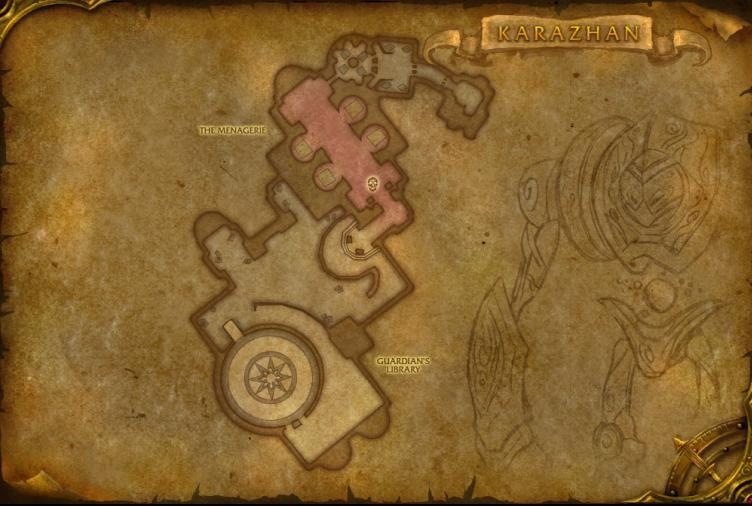
\includegraphics[width=0.85\textwidth]{img/Karazhan/cropped-3457-9.jpg}
\end{center}

The library continues up a ramp at the end of the above region. The ramp contains multiple platforms connected by ramps that lead further up into the castle. One of the bookshelves on the second ramp is rigged with a secret door that can be opened into another chamber. This chamber holds some secret magical scrolls and items. To find this, the party must either stop and take a good look on this ramp freely or roll a 20 on perception while on this ramp.

\begin{center}
	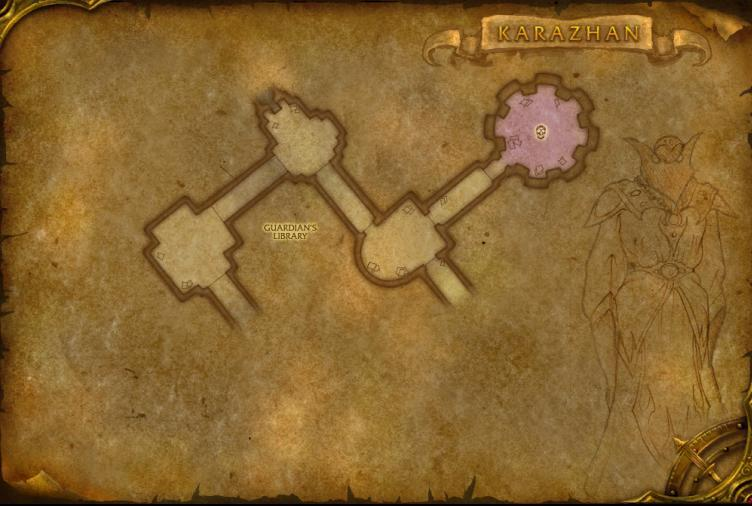
\includegraphics[width=0.48\textwidth]{img/Karazhan/cropped-3457-10.jpg}
	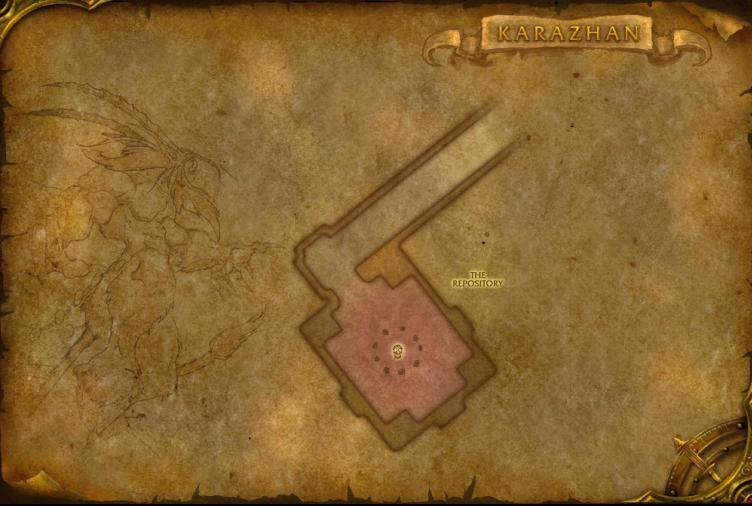
\includegraphics[width=0.48\textwidth]{img/Karazhan/cropped-3457-11.jpg}
\end{center}

\subsubsection{The Observatory}

The observatory is connected to the upper region of the library. The observatory is in one of the highest layers of the castle.

\begin{center}
	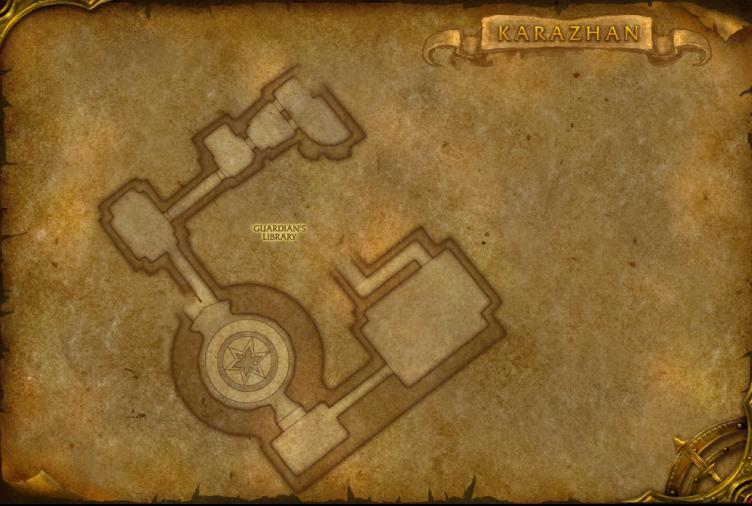
\includegraphics[width=0.48\textwidth]{img/Karazhan/cropped-3457-12.jpg}
	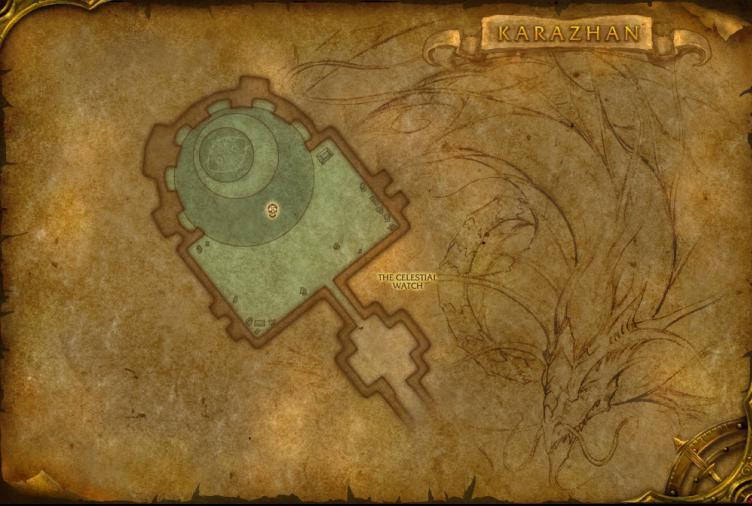
\includegraphics[width=0.48\textwidth]{img/Karazhan/cropped-3457-13.jpg}
\end{center}

Inside of the observatory are many magical items. The observatory is a huge room which houses a ghostly dragon. The dragon is the protector and keeper of the artifacts that can be found in that room. On the door of the observatory is a dragon symbol which serves as warning to those who enter.

\begin{center}
	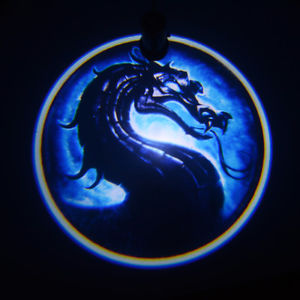
\includegraphics[width=0.39\textwidth]{img/Karazhan/s-l300.jpg}
	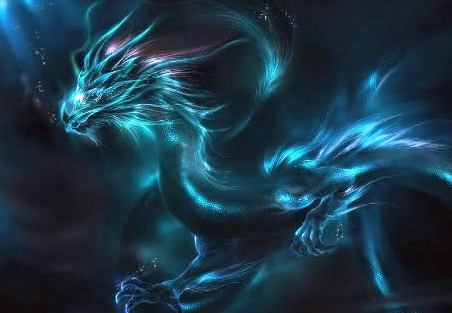
\includegraphics[width=0.57\textwidth]{img/Karazhan/Cloud_dragon.jpg}
\end{center}

\subsubsection{The Chaotic Chess Chamber (Sorcerer's Chess)}

This room contains a large chess board made of the finest marble tiles. The room is surrounded by very well crafted pillars and is perfectly clean as though it had just been polished. The chess board contains large human-size pieces that look like creatures one the black side and it contains a number of empty spaces on the white side equivalent to how many players enter the room. When a player enters a square, they become that piece and the square is locked by a magical barrier. The players essentially enter wizards chess and cannot leave until beating the other side.

\begin{center}
	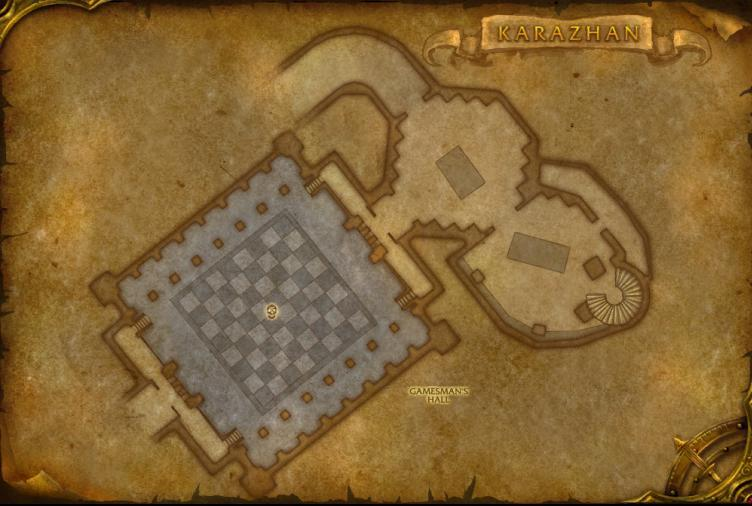
\includegraphics[width=0.48\textwidth]{img/Karazhan/cropped-3457-14.jpg} 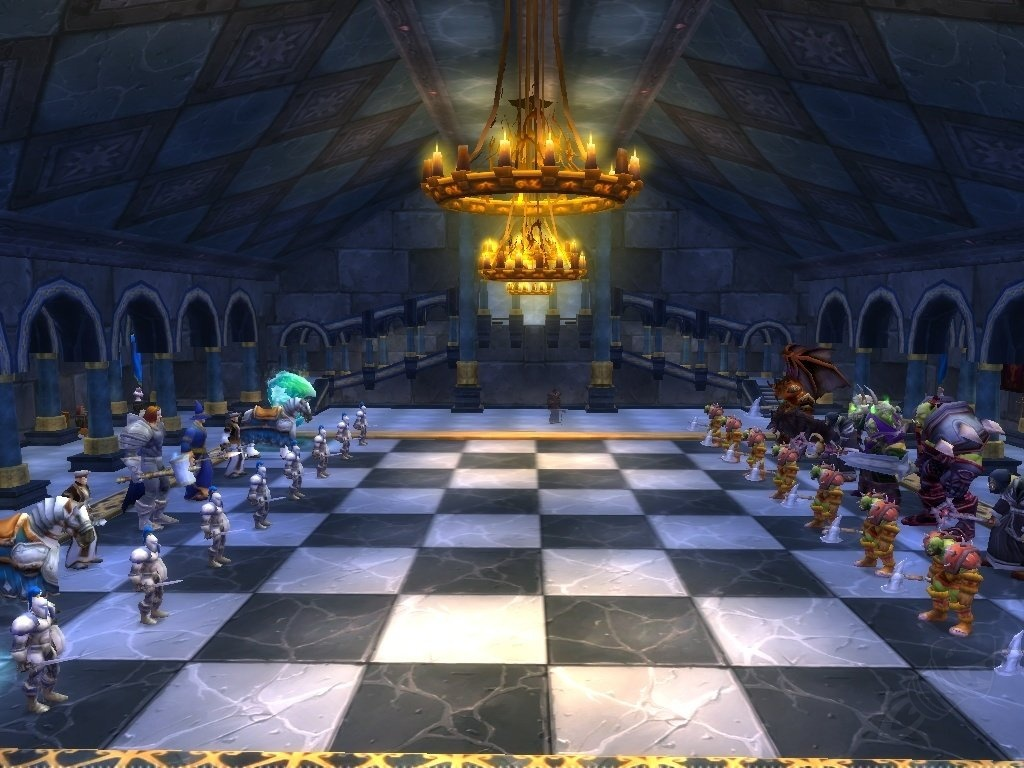
\includegraphics[width=0.43\textwidth]{img/Karazhan/22268-karazhan-gamesmans-hall-this-is-where-you-do-the-chess-event-after-beating-the-e.jpg}
\end{center}

The mechanics of this chess are the players vs the DM. The DM can play at any difficulty level he desires. When a player is removed from the game (the piece is taken), they are knocked to zero hit points and knocked unconscious. They can no longer move and they are teleported off the arena. They will not awakened until healed. There is nothing else in this room other than the chess game, but beating it is the only way to open the door at the end of the room (pass through the room).

\subsubsection{Medivh's Chambers}

Medivh's Chambers are the royal chambers of the castle. This is where Yaga spends her time.

\begin{center}
	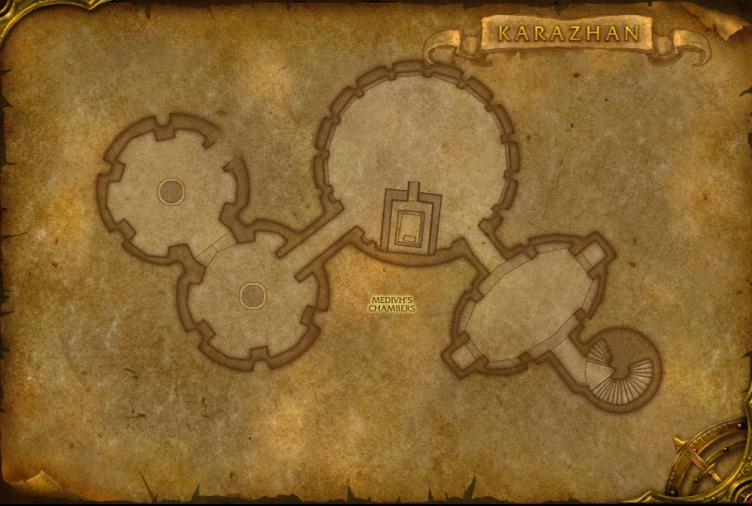
\includegraphics[width=0.48\textwidth]{img/Karazhan/cropped-3457-15.jpg}
	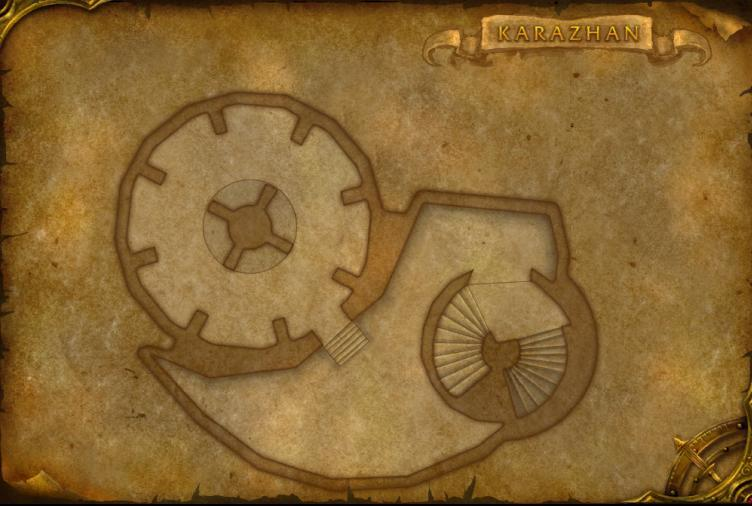
\includegraphics[width=0.48\textwidth]{img/Karazhan/cropped-3457-16.jpg}
\end{center}

\subsubsection{Netherspace}

This is the area on the top of the Karazhan tower. The sky in this region will appear unique and have abstract flows to it that cannot be seen from outside the tower. This is because Yaga (through the Celestials) can peer into other dimensions from this location, which is strongly influenced by the Celestials. When the party arrives at the top (if they do), Yaga will be glancing into an demonic realm (a barren wasteland in a dimension where many demonic beings inhabit).

\begin{center}
	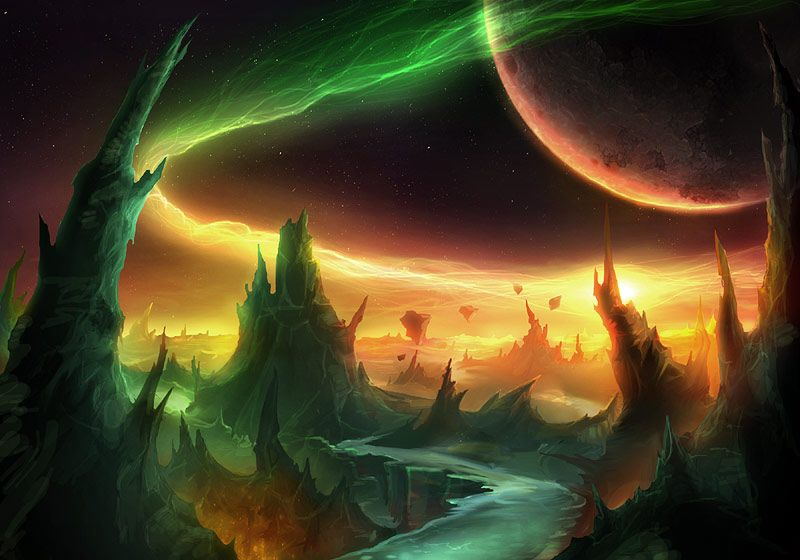
\includegraphics[width=0.47\textwidth]{img/Karazhan/WoW-History-Burning-08.jpg}
	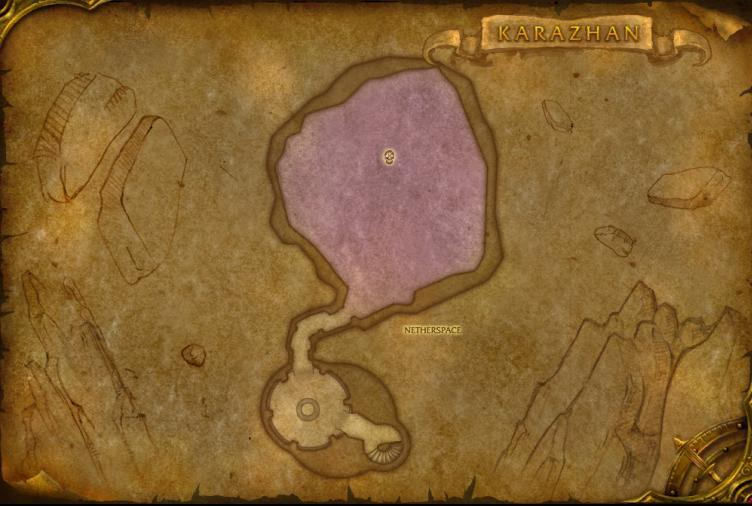
\includegraphics[width=0.49\textwidth]{img/Karazhan/cropped-3457-17.jpg}
\end{center}